\begin{prob}
    
    \begin{center}
	    	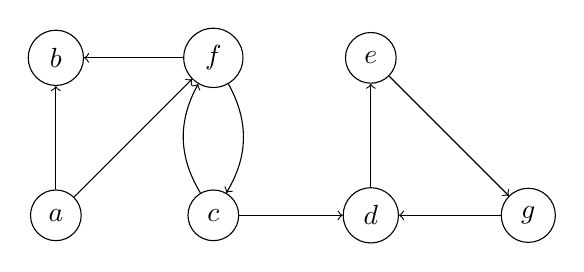
\begin{tikzpicture}
    		    \tikzset{
       			vertex/.style={draw, circle, text width=8, align=center},
        		arc/.style={->}
    		    }
   		        \draw node[vertex] (a) at (0,0) {$a$};
    		    \draw node[vertex] (b) at (0,2) {$b$};
   		        \draw node[vertex] (c) at (2,0) {$c$};
                \draw node[vertex] (f) at (2,2) {$f$};
    		    \draw node[vertex] (d) at (4,0) {$d$};
		        \draw node[vertex] (e) at (4,2) {$e$};
  	            \draw node[vertex] (g) at (6,0) {$g$};
	            \foreach \x/\y in {%
	        	    a/b,a/f,d/e,e/g,f/b,g/d,c/d%
        	    }  
    	        {
       		     	\draw (\x) edge[arc] (\y);
   		        }

                \draw (c) edge[arc, bend left] (f);
                \draw (f) edge[arc, bend left] (c);
		    \end{tikzpicture}
	    \end{center}
    
    \begin{subprobset}
    
        \begin{subprob}
	    	Consider a \emph{breadth}-first search on the graph shown in
        	the figure, starting with node $c$.
        	Which nodes are visited, and in what order? Use the convention
            that graph.neighbors() produces successors in ascending
            order of label.
        \end{subprob}
        
        \begin{soln}
            c,d,f,e,b,g
        \end{soln}

        \vspace{1em}
        
        \begin{subprob}
	        Consider a \emph{breadth}-first search on the graph shown in
	        the figure, starting with node $a$.
            Which nodes are visited, and in what order? Use the convention
            that graph.neighbors() produces successors in ascending
            order of label.
        \end{subprob}
        
        \begin{soln}
            a,b,f,c,d,e,g
        \end{soln}

        \vspace{1em}
        
        \begin{subprob}
	        Consider a \emph{breadth}-first search on the graph shown in
    	    the figure, starting with node $g$.
            Which nodes are visited, and in what order? Use the convention
            that graph.neighbors() produces successors in ascending
            order of label.
        \end{subprob}
        
        \begin{soln}
            g,d,e
        \end{soln}

        \vspace{1em}
            
    \end{subprobset}

\end{prob}
